\documentclass[letterpaper]{article}
\usepackage[empty]{fullpage}
\usepackage{color}
\usepackage[pdftex]{graphicx}
\definecolor{blue}{RGB}{1,77,255}
\addtolength{\oddsidemargin}{-0.375in}
\addtolength{\evensidemargin}{0.375in}
\addtolength{\textwidth}{0.5in}
\addtolength{\topmargin}{-0.375in}
\addtolength{\textheight}{0.75in}
\raggedright

\graphicspath{{./images/}}

\begin{document}

\tableofcontents
\listoffigures

\eject

\section{Introduction}

\subsection{Purpose}

The purpose of this document is four-fold:

\begin{enumerate}
\item  Define a full set of requirements for the IM-Net. (These sections correspond to a Software Requirements Document (SRD)).

\item  Define the design for the IM-Net. (These sections correspond to a Software Design Document (SDD)).

\item  Define the Test Plan for the IM-Net. (These sections correspond to a Software Test Plan (STP)).

\item  Define and partially implement feasible modules for the IM-Net.  (These sections correspond to the Software Implementation Document (SID)).
\end{enumerate}

The complete definition of all IM-Net requirements provides the source requirement inputs for the development of the subsequent supporting software subsystems documents.

\subsection{Scope}

The documentation developed as part of this CS437 class, starts from the SRD prepared in CS337 or in previous CS437 classes with a much reduced scope.  The scope of this document includes the following:

\begin{enumerate}
\item  All functional and non-functional requirements on the IM-Net are captured.  This includes Verification \& Validation (V\&V) requirements, as well as inter-software subsystems requirements.

\item  A complete set of IM-Net Requirements, derived and traceable to the incoming class requirements.  These requirements are organized by key IM-Net functional units shown on the Level 1 DFD given in section 2.0.

\item  A trace matrix, relating all IM-Net functional requirements to functional subunits as expanded in lower level DFDs. Higher level DFDs are provided as part of the design in section 4.0

\item  The functional requirements defined in the IM-Net Requirements section have been expanded to include more specific hardware requirements.
\end{enumerate}

\subsubsection{Organization}

The organization of this document provides a natural 'flow' or allocation of requirements to each succeeding section. Details regarding the overall document structure are discussed in sub-section 1.4.

\subsubsection{Relationship to Other Documents}

The IM-Net SRD/SDD/STP/SID is a complete self contained document. Some relationships to other documents in the literature are indicated below in sub-section 1.5.

\subsection{Project Name Architecture}
 
\subsubsection{Detailed Context Diagram (DFD Level 0)}

The IM-Net architecture is summarized in the Context Diagram (DFD Level 0) given below. A more detailed Functional Description is given in Section 2 of this document.\\

% Note: All image files should have a width < 7.75in
\begin{figure}[h]
\centering
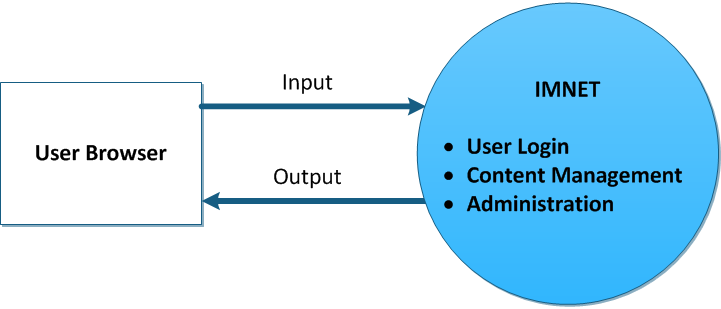
\includegraphics{DFD_level_0}
\caption{Context Diagram (DFD Level 0)}
\label{fig:DFD_level_0}
\end{figure}
\eject

The foremost objective of IM-Net is to assist music artists, label and venues in reaching out to their fans through a vibrant, web-based, multimedia interface.

IM-Net is a software application which provides major functions such as the ones listed below:

\begin{enumerate}
\item  Provides a portal for independent music artists, labels and venues to connect with their fans.

\item  The ability for artists and label to upload and showcase their music to their fans.

\item  Allows music artists, labels and venue to connect to their fans through the messaging interface.
\end{enumerate}

IM-Net is implemented primary using the Django content management system, a web-based framework that closely follows the Model-View-Controller architectural pattern. Data models are framed using Python classes and are stored into a SQL relational database. Views are implemented using Django's Template language, which are used by Django to generate dynamic HTML output. Controllers are Python scripts that describe to the view which particular data will be shown. 

TODO: WRITE MORE HERE

\subsection{Documentation Development Process}

The IM-Net detailed functional description is documented in section 2.0. Basically, Section 2 is a succinct software description document. The overall detailed functional description is based on higher level DFDs (above level 1). All major functional units are described in detail in this part of the document.

Requirements affecting the IM-Net are captured in Section 3.0 of this document.  These requirements are a refinement and completion of requirements first collected as part of a previous Software Engineering project. The document is cited in Section 1.2.2. This section is the one worked in most detail to become a reasonably complete Software Requirements Document (SRD). It includes both functional and non-functional software requirements together with several detailed ``rational'' paragraphs whenever necessary to complete the understanding of each requirement.

Section 4 is the IM-Net detailed Design Description Document (SDD). This part of the document includes all higher level DFDs as described in section 2 plus all interface units. The document is highly technical and it is based on section 2 descriptions. An important component is the addition of a SIS (software interface specification) document in sub-section 4.2.

Section 5 includes elements of a partial implementation of the IM-Net. This section includes the various constraints that effectively limit the implementation as well as the sub-units that will be coded. The implementation goals are defined and the code and pseudo code are included as an attachment to this section.  

Section 6 is the last major section in this document and includes the overall Test Plan (TP) of the IM-Net. The test plan details the various techniques used to test the requirements and it also includes a Validation Matrix where each requirement specified in section 3 is listed with its corresponding validation method. In addition, TP specifies the mandated peer reviews needed to validate the stakeholders part of the requirements.

 
\subsection{References}

All references used in the creation of this document are listed below.

\subsubsection{Controlling Documents}

There is no document controlling this document.

\subsubsection{Applicable Documents}

No addition applicable document has been used in the production of this document.

\subsubsection{Standards}

No Standard has been used in the creation of this document. However, some Standards described in textbooks have been examined as a reference. In particular, the IEEE standard has been briefly discussed in class.

\eject

\section{Detailed Function Description of IM-Net}

\subsection{Detailed IM-Net Functional Description}

\subsubsection{High Level DFDs}

The IM-Net major functional subunits are shown in the DFD Level 1 depicted below:

\begin{figure}[h!]
\centering
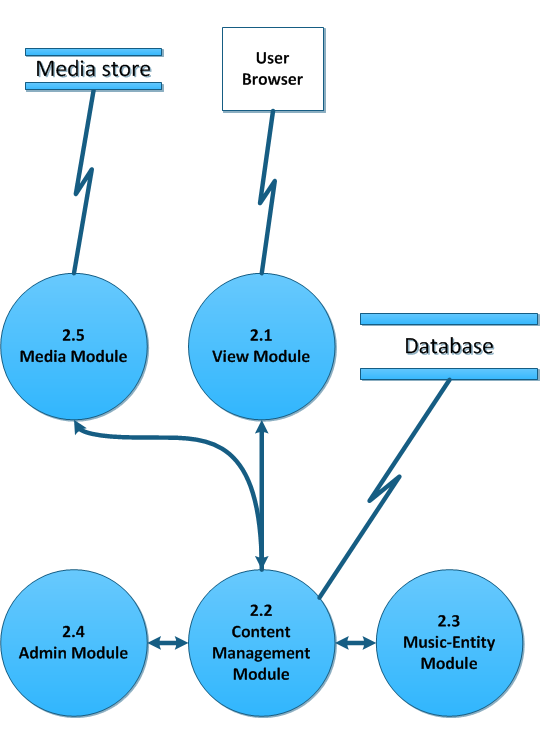
\includegraphics{DFD_level_1.png}
\caption{DFD Level 1}
\label{fig:DFD_level_1}
\end{figure}
\eject
 
\subsubsection{Detailed Functional Description of the IM-Net Major Units}

The description of the function of the IM-Net major functional units shown in Figure 2-X follows.

\eject

\section{The IM-Net Requirements}
 
\subsection{IM-Net Functional Requirements}

This Section collects all the IM-Net Functional Requirements. This section includes the complete set of functional requirements with explanation and rational where the statement of the requirement was deemed insufficient or needing additional background/justification. All requirements relate to the design modules described in Section 2. An effort has been made to standardize the correlation between the design modules and the requirements to make their access and organization more consistent. For example, requirement number ``n'' affecting module 2.1 will be labeled 3.1-n.

\textbf{TODO: WRITE FUNCTIONAL REQUIREMENTS}\\

\subsection{IM-Net Non-Functional Requirements}

This Section collects all the IM-Net Non-Functional Requirements. All non-functional requirements are numbered ``NF -- n'' where ``n'' indicates the n${}^{th}$ requirement.

\begin{enumerate}
\item  IM-Net shall require minimal training for users who have experience with common web browsers and web-based applications.

\item  IM-Net shall not disclose any personal information about any artists, label, venue or fan to unauthorized users.

\item  IM-Net shall be rapidly deployable to any Apache/SQL/Python/Django software stack.

\item  IM-Net shall  \#4

\item  IM-Net Non Functional Requirement \#5
\end{enumerate}

\subsection{IM-Net Hardware Requirements}

This Section collects all the IM-Net Hardware Requirements. All hardware requirements are numbered ``H -- n'' where ``n'' indicates the n${}^{th}$ requirement.

\begin{enumerate}
\item  IM-Net requires an scalable compute cloud instance.

\item  IM-Net Hardware Requirement \#2

\item  IM-Net Hardware Requirement \#3

\item  IM-Net Hardware Requirement \#4

\item  IM-Net Hardware Requirement \#5
\end{enumerate}

\eject

\section{IM-Net Detailed Design}

In this section, the IM-Net described in Section 2 with requirements listed in Section 3 will be designed in detail including several higher level DFDs. Each major module detailed design is included in correspondence with the design sections defined in Section 2 and responding to the requirements listed in its correlated sub-section in chapter 3.

The detailed design of each of the four modules discussed in section 2 with requirements presented in section 3 is presented in Figures 4-1, 4-2, 4-3, and 4-4. As done in previous cases, Figure 4-1 corresponds to the detailed design of Module 2.1, and so on.

Figure 4-1 shows the four sub-modules that comprise module 2.1. Next, Figure 4-2 shows the three sub-modules that comprise module 2.2. Then, Figure 4-3 shows the four sub-modules that comprise module 2.3. Lastly, Figure 4-4 depicts the three sub-modules that comprise module 2.4.

\eject 

 
\section{IM-Net Elements of Implementation}

In this section (some of) the modules designed in Section 4 with requirements listed in Section 3 will be implemented initially at least at the level of pseudo code. Where possible, actual code will be provided. Each module is implemented in correspondence with the design sections defined in section 2 and responding to the requirements listed in its correlated sub-section in chapter 3.

\eject 

\section{IM-Net Test Plan}

\subsection{Introduction}

In this section the testing methodology to be used to Verify and Validate each of the requirements listed in section 3.0 has been identified. At points some additional testing may be required and they shall be documented as an attachment to this document. 

The methodologies and testing strategies identified at this point include three major approaches with various variations to adapt to the IM-Net project:

\begin{enumerate}
\item  Testing using addition ad-hoc crated software including a correlation testing unit.

\item  Demonstration of the specified capability

\item  Inspection of the software code possibly using addition inspection techniques
\end{enumerate}

 
\subsection{Functional Requirements Validation Matrix}
The IM-Net Functional and Performance Requirements Validation Matrix is given below.
\eject 
 
\section{Acronyms}
\textbf{IM-Net}  Independent Music Network

\eject 
 
\section{Data Dictionary}

\underbar{Item 1}: Description. 

\end{document}
